% !TEX root = Paper.tex
% !TEX root = Paper.tex
\documentclass[conference]{IEEEtran}
\IEEEoverridecommandlockouts
% The preceding line is only needed to identify funding in the first footnote. If that is unneeded, please comment it out.
\usepackage{cite}
\usepackage[T1]{fontenc}
\usepackage{amsmath,amssymb,amsfonts}
\usepackage{algorithmic}
\usepackage{graphicx}
\usepackage{textcomp}
\usepackage{xcolor}
\usepackage{hyperref}
\usepackage{cleveref}
\usepackage{tikz}
\usepackage{pgfplots}
% !TEX root = Paper.tex
\pgfplotsset{compat=1.18}
\def\BibTeX{{\rm B\kern-.05em{\sc i\kern-.025em b}\kern-.08em
    T\kern-.1667em\lower.7ex\hbox{E}\kern-.125emX}}

\makeatletter
\newcommand{\linebreakand}{%
  \end{@IEEEauthorhalign}
  \hfill\mbox{}\par
  \mbox{}\hfill\begin{@IEEEauthorhalign}
}
\makeatother
\begin{document}

\title{Unified State Feedback Control of a Hybrid Distribution Transformer using Particle Swarm Optimization\\
% \thanks{Identify applicable funding agency here. If none, delete this.}
}

\author{\IEEEauthorblockN{1\textsuperscript{st} Dave Figueroa}
\IEEEauthorblockA{\textit{Institute of Control and Industrial Electronics} \\
\textit{Warsaw University of Technology}\\
Warsaw, Poland \\
email address or ORCID}
\and
\IEEEauthorblockN{2\textsuperscript{nd} Jun Cheng}
\IEEEauthorblockA{\textit{Research Institute of Interdisciplinary Intelligent Science} \\
\textit{Ningbo University of Technology}\\
Ningbo, China \\
email address or ORCID}
\and
\IEEEauthorblockN{3\textsuperscript{nd} Zhihong Zhao}
\IEEEauthorblockA{\textit{Research Institute of Interdisciplinary Intelligent Science} \\
\textit{Ningbo University of Technology}\\
Ningbo, China \\
email address or ORCID}
\and
\IEEEauthorblockN{4\textsuperscript{nd} Alvaro Carreno}
\IEEEauthorblockA{\textit{Institute of Control and Industrial Electronics} \\
\textit{Warsaw University of Technology}\\
Warsaw, Poland \\
email address or ORCID}
\and
\IEEEauthorblockN{5\textsuperscript{rd} Mariusz Malinowski}
\IEEEauthorblockA{\textit{Institute of Control and Industrial Electronics} \\
\textit{Warsaw University of Technology}\\
Warsaw, Poland \\
email address or ORCID}
}

\maketitle

\begin{abstract}
Here will be the abstract of the paper.
\end{abstract}

\begin{IEEEkeywords}
    hybrid distribution transformer, optimal control, particle swarm optimization
\end{IEEEkeywords}

\section{Introduction}

% !TEX root = Paper.tex
\IEEEPARstart{T}{he} increasing penetration of renewable energy sources in the electrical grid has led to a significant rise in the use of power electronic converters. These converters are essential for integrating RES into the grid, as they facilitate the conversion of DC power generated by sources like solar panels and wind turbines into AC power compatible with the grid~\cite{Blaabjerg2023}. However, the widespread use of power electronic converters has also introduced challenges related to power quality, such as the injection of harmonics and non-linear loads, which can lead to voltage distortions and other issues in the electrical grid~\cite{Najafzadeh2021,Sepasi2023}.

There are many solutions that have been proposed to address the power quality issues in the grid, such as static compensators (STATCOMs)~\cite{Engelbrecht2023}, dynamic voltage restorers (DVRs)~\cite{Kandil2020}, active power filters (APFs)~\cite{Mishra2020}, unified power quality conditioners (UPQC)~\cite{Fujita1998} and the solid-state transformers (SST)~\cite{Huber2019}. SSTs has the ability to mitigate most of the power quality issues mentioned above, while also providing galvanic isolation and voltage transformation. However, the high cost and complexity of SSTs has limited their widespread adoption in the distribution grid and, also, does not provide the same short-circuit current capability as traditional distribution transformers (DTs)~\cite{carrenoConfigurationsPowerTopologies2021}.

For this reason, the hybrid distribution transformer (HDT) emerges as a promising solution to address the disadvantages of SSTs while still providing advanced power quality functionalities.
The HDT is a power electronic transformer that combines the functions of a traditional distribution transformer with those of power electronic converters~\cite{haj-maharsiHybridDistributionTransformer2010,matelskiBadaniaEksperymentalneTransformatora2023}. Many HDT configurations have been proposed in the literature, and in consequence, classifications have been made~\cite{carrenoConfigurationsPowerTopologies2021}. One of the classifications is based on the source of the converter's energy, i.e., whether the energy is obtained from a capacitor/battery, the primary or secondary side of the DT, or an auxiliary winding. On the other hand, the other classification is based on how the converters inject energy into the system, i.e., whether they are connected in series or in parallel with the DT. 

In this paper, the configuration of the HDT consists of the DT connected to two back-to-back voltage source converters (VSCs): a series converter connected to the primary of the DT through a coupling transformer (CT), and a parallel converter connected in parallel to the load, which is connected to the secondary of the DT. A circuit diagram of the HDT is shown in \cref{fig:HDT_Transformer}. The series converter is responsible for regulating the voltage at the primary side of the DT, while the parallel converter is responsible for regulating the current injected into the load.

Several control strategies have been proposed for the HDT in the literature, including finite control set model predictive control (FCS-MPC)~\cite{costaFourlegMatrixConverter2022}, switching V-f and P-Q mode control~\cite{xuThreePhaseHybridTransformer2023}, and decoupled control strategies, such as the resonant control~\cite{matelskiBadaniaEksperymentalneTransformatora2023} the compound controller~\cite{liuCompoundControlSystem2020}, quasi-proportional controller~\cite{liuQuasiProportionalResonantControlHybrid2022} and the separated state-feedback controller~\cite{carrenoStateFeedbackControlHybrid2024}.

In this paper, a unified control strategy based on state feedback control with resonant states is proposed for the HDT. This control strategy aims to achieve zero steady-state error for sinusoidal references and disturbances, while also ensuring good dynamic performance. The control strategy is designed using an augmented state-space model of the HDT that includes the delays introduced by the digital control system and the resonant states to achieve zero steady-state error for sinusoidal references and disturbances. The control gains are optimized using particle swarm optimization (PSO), which had been previously used for tuning the control gains of state-feedback controllers in power electronic converters~\cite{ufnalskiParticleSwarmOptimization2015}. The PSO algorithm is used  to minimize a cost function that considers both the transient and steady-state performance of the HDT. The proposed control strategy is validated through simulation results that demonstrate its effectiveness in regulating the voltage and current of the HDT under various operating conditions.

\section{Model of the Hybrid Distribution Transformer}

\subsection{Series Converter}

\begin{align}
    \begin{aligned}
        v_s &= R_{fs}i_{fs} + L_{fs}\dfrac{d\,i_{fs}}{dt} + v_{cs} \\
        i_{fs} &= C_{fs}\dfrac{d\,v_{cs}}{dt} + i_g \\
    \end{aligned}
\end{align}

Leaving the states on the left side, and converting to $\alpha\beta$ coordinates, the series converter model is given by:

\begin{align}
    \begin{aligned}
        \dfrac{d\,i_{fs}}{dt} &= -\dfrac{R_{fs}}{L_{fs}}i_{fs} - \dfrac{1}{L_{fs}}v_{cs} + \dfrac{1}{L_{fs}}v_s \\
        \dfrac{d\,v_{cs}}{dt} &= -\dfrac{1}{C_{fs}}i_{fs} + \dfrac{1}{C_{fs}}i_g
    \end{aligned}
\end{align}

\subsection{Parallel Converter}

\begin{align}
    \begin{aligned}
        v_p &= R_{fp}i_{fp} + L_{fp}\dfrac{d\,i_{fp}}{dt} + v_{cp} \\
        i_{fp} &= C_{fp}\dfrac{d\,v_{cp}}{dt} - i_Y + i_L
    \end{aligned}
\end{align}

Leaving the states on the left side, and converting to $\alpha\beta$ coordinates, the series converter model is given by:

\begin{align}
    \begin{aligned}
        \dfrac{d\,i_{fp}}{dt} &= -\dfrac{R_{fp}}{L_{fp}}i_{fp} - \dfrac{1}{L_{fp}}v_{cp} + \dfrac{1}{L_{fp}}v_p \\
        \dfrac{d\,v_{cp}}{dt} &= \dfrac{1}{C_{fp}}i_{fp} - \dfrac{1}{C_{fp}}i_Y + \dfrac{1}{C_{fp}}i_L
    \end{aligned}
\end{align}

\subsection{Distribution Transformer}

The transformer is connected in $\Delta-Y$ configuration, with the series converter connected to the delta side, and the parallel converter connected to the $Y$ side. The transformer equations are given by:

\begin{align}
    \begin{aligned}
        v_{Ya} &= N_{LFT}(v_{\Delta a} - v_{\Delta b}) \\
        v_{Yb} &= N_{LFT}(v_{\Delta b} - v_{\Delta c}) \\
        v_{Yc} &= N_{LFT}(v_{\Delta c} - v_{\Delta a})
    \end{aligned}
\end{align}
This can be expressed in matrix form as:
\begin{align}
    \begin{aligned}
        v_Y &= N_{LFT}
        \underbrace{
        \begin{bmatrix}
            1 & -1 & 0 \\
            0 & 1 & -1 \\
            -1 & 0 & 1
        \end{bmatrix}
        }_{K_T'}
        v_{\Delta}\\
        v_Y &= N_{LFT} K_T' v_{\Delta}
    \end{aligned}
\end{align}
The dynamics of the transformer can be expressed as:
\begin{align}
    v_{Y} &= R_Yi_Y + L_Y\dfrac{d\,i_Y}{dt} + v_{cp} \\
    \intertext{Assuming that there is no zero-sequence current, the transformer model can be expressed in $\alpha\beta$ coordinates as:}
    \dfrac{d\,i_Y}{dt} &= -\dfrac{R_Y}{L_Y}i_Y - \dfrac{1}{L_Y}v_{cp} + \dfrac{1}{L_Y}N_{LFT}K_T'v_{\Delta}
\end{align}

\subsection{Overall HDT Model}
The overall HDT model can be expressed in state-space form as:
\begin{align}
    \begin{aligned}
        \dfrac{d}{dt}
        \begin{bmatrix}
            x_s\\
            x_p
        \end{bmatrix}
        &=
        \begin{bmatrix}
            \mathbf{A}_s & \mathbf{P}_{ig}\mathbf{M}_p \\
            \mathbf{P}_{vc}\mathbf{M}_s & \mathbf{A}_p
        \end{bmatrix}
        \begin{bmatrix}
            x_s\\
            x_p
        \end{bmatrix}
        +
        \begin{bmatrix}
            \mathbf{B}_s & \mathbf{0} \\
            \mathbf{0} & \mathbf{B}_p
        \end{bmatrix}
        \begin{bmatrix}
            u_s\\
            u_p 
        \end{bmatrix}
        \\
        &+
        \begin{bmatrix}
            \mathbf{0}\\
            \mathbf{P}_{vg}
        \end{bmatrix}
        v_g
        +
        \begin{bmatrix}
            \mathbf{0}\\
            \mathbf{P}_{iL}
        \end{bmatrix}
        i_L
    \end{aligned}
\end{align}
where the matrices $\mathbf{M}_p = \begin{bmatrix}\mathbf{0} & \mathbf{I} & \mathbf{0}\end{bmatrix}$ and $\mathbf{M}_s = \begin{bmatrix}\mathbf{0} & \mathbf{I}\end{bmatrix}$ are used to select the appropriate states from the parallel and series converter state vectors respectively.

\section{Control Strategy}

Withe the state-space model of the HDT defined, the next step is to design a control strategy that ensures the desired performance. The proposed control strategy is based on a state feedback controller with integral action and resonant states to achieve zero steady-state error for sinusoidal references and disturbances. The block diagram of the proposed control strategy is shown in Fig. \ref{fig:Control_Diagram}.

\begin{equation}
    u_k = -\mathbf{K}_x \mathbf{H}_a
    \begin{bmatrix}
        x_k\\
        m_k
    \end{bmatrix} + \mathbf{K}_{err}e_k - \mathbf{K}_r \rho_k + \mathbf{K}_u m_k
\end{equation}
where $\mathbf{K}_x$ is the state feedback gain matrix, $\mathbf{H}_a$ is the matrix that selects the states without reference, $\mathbf{K}_{err}$ is the error gain matrix, $e_k$ is the error vector, $\mathbf{K}_r$ is the resonant states gain matrix, $\rho_k$ is the resonant states vector, $\mathbf{K}_u$ is the previous control input gain matrix, and $u_{k - 1}$ is the previous control input vector.

\begin{figure}[t!]
    \centering
    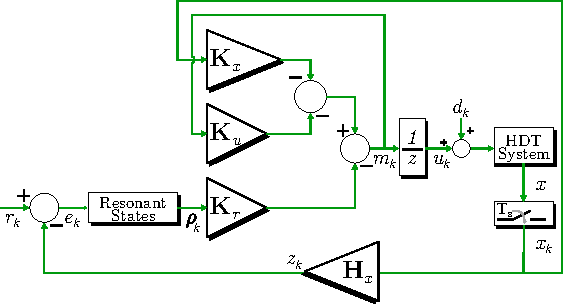
\includegraphics[width=\columnwidth]{Images/Control_Diagram.pdf} 
    \caption{Block diagram of the proposed control strategy for the HDT.}
    \label{fig:Control_Diagram}
\end{figure}

The resonant states are included to ensure zero steady-state error for sinusoidal references and disturbances. The resonant states dynamics are given by:
\begin{equation}
    \dfrac{d\,\rho(t)}{dt} = 
    \underbrace{
    \begin{bmatrix}
        -2\xi\omega & \omega \\
        -\omega & 0
    \end{bmatrix}
    }_{\mathbf{A}_r}
    \rho(t) + 
    \underbrace{
    \begin{bmatrix}
        1\\
        0
    \end{bmatrix}
    }_{\mathbf{B}_r}
    e(t)
\end{equation}
where $\omega$ is the nominal angular frequency, $\xi$ is the damping factor. Each of the references signals has two resonant states associated with it, meaning that for the HDT control, there are eight resonant states in total (4 for the $ev_{cs,\alpha\beta}$ and 4 for the $i_{fp,\alpha\beta}$). This can be expressed as:
\begin{align}
    \dfrac{d\,\rho(t)}{dt} &= \text{blkdiag}(\mathbf{A}_r, \mathbf{A}_r, \mathbf{A}_r, \mathbf{A}_r)\rho(t)\\
    &+ \text{blkdiag}(\mathbf{B}_r, \mathbf{B}_r, \mathbf{B}_r, \mathbf{B}_r)e(t)
\end{align}

These resonant states are then discretized using a ZOH giving the matrices $\mathbf{A}_{rd}$ and $\mathbf{B}_{rd}$. The augmented state-space model of the resonant states can be expressed as:
\begin{align}
    \begin{aligned}
        \begin{bmatrix}
            x_{k + 1}\\
            m_{k + 1}\\
            \rho_{k + 1}
        \end{bmatrix}
        &=
        \begin{bmatrix}
            \mathbf{A}_{d,delay} & \mathbf{0} \\
            \mathbf{B}_{rd}\mathbf{H}_x & \mathbf{A}_{rd}
        \end{bmatrix}
        \begin{bmatrix}
            x_k\\
            m_k\\
            \rho_k
        \end{bmatrix}
        +
        \begin{bmatrix}
            \mathbf{B}_{d,\text{aug}}\\
            \mathbf{0}
        \end{bmatrix}
        \begin{bmatrix}
            u_k\\
            e_k
        \end{bmatrix}
        \\
        y_k &= 
        \begin{bmatrix}
            \mathbf{C} & \mathbf{0}
        \end{bmatrix}
        \begin{bmatrix}
            x_K\\
            m_k\\
            \rho_k
        \end{bmatrix}
    \end{aligned}
\end{align}
where $\mathbf{H}_x$ selects the states from the HDT state vector that are imposed to follow references.

\subsection{Particle Swarm Optimization}

The PSO algorithm is a population-based optimization technique inspired by the social behavior of birds and fish. It consists of a swarm of particles, where each particle represents a potential solution to the optimization problem. The particles move through the search space, updating their positions based on their own experience and the experience of their neighbors. The velocity and position of each particle are updated using the following equations:
\begin{align}
    \begin{aligned}
        v_j(i + 1) &= K_{ap}\left(v_j(i) + c_1 r_1 (pbest_j - x_j(i)) \right.\\
        & \left. + c_2 r_2 (gbest - x_j(i))\right)\\
        x_j(i + 1) &= x_j(i) + v_j(i + 1)
    \end{aligned}
\end{align}
where $v_j(i)$ is the velocity of particle $j$ at iteration $i$, $x_j(i)$ is the position of particle $j$ at iteration $i$, $pbest_j$ is the best position found by particle $j$, $gbest$ is the best position found by the entire swarm, $c_1$ and $c_2$ are cognitive and social acceleration coefficients, $r_1$ and $r_2$ are random numbers uniformly distributed in the range [0, 1], and $K_{ap}$ is the constriction factor given by:
\begin{equation}
    K_{ap} = \dfrac{2}{\left|2 - \phi - \sqrt{\phi^2 - 4\phi}\right|}
\end{equation}
where $\phi = c_1 + c_2 > 4$ is a constant that ensures convergence.

The PSO algorithm iteratively updates the positions and velocities of the particles until a stopping criterion is met, such as a maximum number of iterations or a satisfactory solution. The best position found by the swarm is considered the optimal solution to the optimization problem.

\section{Simulation Results}

% !TEX root = Paper.tex

In this section, the simulation results of the proposed control strategy are presented. The simulations are performed using MATLAB/Simulink, and the system parameters are listed in Table \ref{tab:params}. The proposed control strategy is tested under grid unbalanced swell, load impact, load unbalance, and non-linear load conditions.

\begin{table}[h!]
    \centering
    \caption{System Parameters}
    \begin{tabular}{|c|c|c|}
        \hline
        Parameter & Variable & Value \\
        \hline
        \hline
        Grid Voltage & $V_{g}$ & 10 kV \\
        Nominal Converter Voltage & $V_s$ & 400 V \\
        DC Link Voltage & $V_{DC}$ & 700 V \\
        Grid Frequency & $f_e$ & 50 Hz \\
        Series Converter Filter Inductance & $L_{fs}$ & $200\ \mu\text{H}$ \\
        Series Converter Filter Resistance & $R_{fs}$ & $100\ \text{m}\Omega$ \\
        Series Converter Filter Capacitance & $C_{fs}$ & $12\ \mu\text{F}$ \\
        Parallel Converter Filter Inductance & $L_{fp}$ & $200\ \mu\text{H}$ \\
        Parallel Converter Filter Resistance & $R_{fp}$ & $100\ \text{m}\Omega$ \\
        Parallel Converter Filter Capacitance & $C_{fp}$ & $12\ \mu\text{F}$ \\
        Transformer Dispersion Inductance & $L_Y$ & $100\ \mu\text{H}$ \\
        Transformer Series Resistance & $R_Y$ & $5\ \text{m}\Omega$\\
        Coupling Transformer Turns Ratio & $N_{CT}$ & $5$ \\
        Distribution Transformer Turns Ratio & $N_{DT}$ & $V_s/(V_g\sqrt{3})$ \\
        Converters Switching Frequency & $f_{\text{sw}}$ & 20 kHz \\
        Control Sampling Time & $T_s$ & 50 µs \\
        \hline
    \end{tabular}
    \label{tab:params}
\end{table}

Each of the load impacts are comprised by $47\ \Omega$ resistive load per phase, $2\ k\Omega$ resistive load in phase $a$ for the unbalanced load, and a three-phase diode bridge rectifier with a $47\ \Omega$ resistive load at its output for the non-linear load. The simulation results are shown in \Cref{fig:Sim_results}.

\subsection{Grid Voltage Unbalanced Swell Compensation}

In the instant $t=10\ ms$ until the instant $t = 260\ ms$ as it can be seen in the \Cref{fig:Sim_results}.(a). The proposed control strategy effectively compensates for the unbalanced swell, meaning that the parallel inverter injects the necessary voltage to maintain a balanced transformer secondary side current, as shown in \Cref{fig:Sim_results}.(d) for the transformer secondary side current and in \Cref{fig:Sim_results}.(c) for the parallel inverter voltage. 

\subsection{Load Impact and Unbalanced Load Compensation}

At $t=60\ ms$, a three-phase balanced load impact is applied, and at $t=100\ ms$, a three-phase unbalanced load is applied, where the resistor of the phase $a$ is $2\ k\Omega$, as shown in \Cref{fig:Sim_results}.(b). To keep a balanced transformer secondary side current, the parallel converter injects the needed current, giving the desired performance, as shown in \Cref{fig:Sim_results}.(d)

\subsection{Non-linear Load Compensation}

Following the load impacts, at $t=140\ ms$, a non-linear load is applied, as it shown in the \Cref{fig:Sim_results}.(b), which consists of a three-phase diode bridge rectifier with a resistive load of $47\ \Omega$ at its output. The parallel converter compensates for the harmonics injected by the non-linear load, giving the secondary side currents that are shown in the \Cref{fig:Sim_results}.(d).

\subsection{Grid Harmonics Compensation}

Finally, at $t=200\ ms$, a third-order harmonic is added to the grid voltage, as shown in \Cref{fig:Sim_results}.(a). The parallel converter compensates for the harmonic distortion, giving the series converter capacitor voltage shown in \Cref{fig:Sim_results}.(c).

\section{Conclusions}

% Use \eqref{label}

% Please don't use the \verb|{eqnarray}| equation environment. Use
% \verb|{align}| or \verb|{IEEEeqnarray}| instead. The \verb|{eqnarray}|
% environment leaves unsightly spaces around relation symbols.

% \item The prefix ``non'' is not a word; it should be joined to the word it modifies, usually without a hyphen.
% \item There is no period after the ``et'' in the Latin abbreviation ``et al.''.

\bibliographystyle{IEEEtran}
\bibliography{bib.bib}

\end{document}
